% Proposed architecture, drawn in TikZ. Compile with pdfLaTeX.
% Graph attention, pre-normalization and residual blocks are illustrative design choices.
\documentclass[11pt]{article}
\usepackage[paperwidth=20cm,paperheight=16.5cm,margin=5mm]{geometry}
\usepackage[T1]{fontenc}
\usepackage{lmodern,amssymb}
\usepackage{tikz,amsmath}
\usetikzlibrary{arrows.meta,calc}
\pagestyle{empty}
\definecolor{outline}{HTML}{153543}
\definecolor{norm}{HTML}{B9CDD0}
\definecolor{attn}{HTML}{ECE6D8}
\definecolor{ffn}{HTML}{B9B2C4}
\definecolor{linear}{HTML}{D8B5BE}
\definecolor{output}{HTML}{DDD7D1}
\definecolor{comp}{HTML}{A8D5CE}
\definecolor{analog}{HTML}{C9BEDA}
\begin{document}
\noindent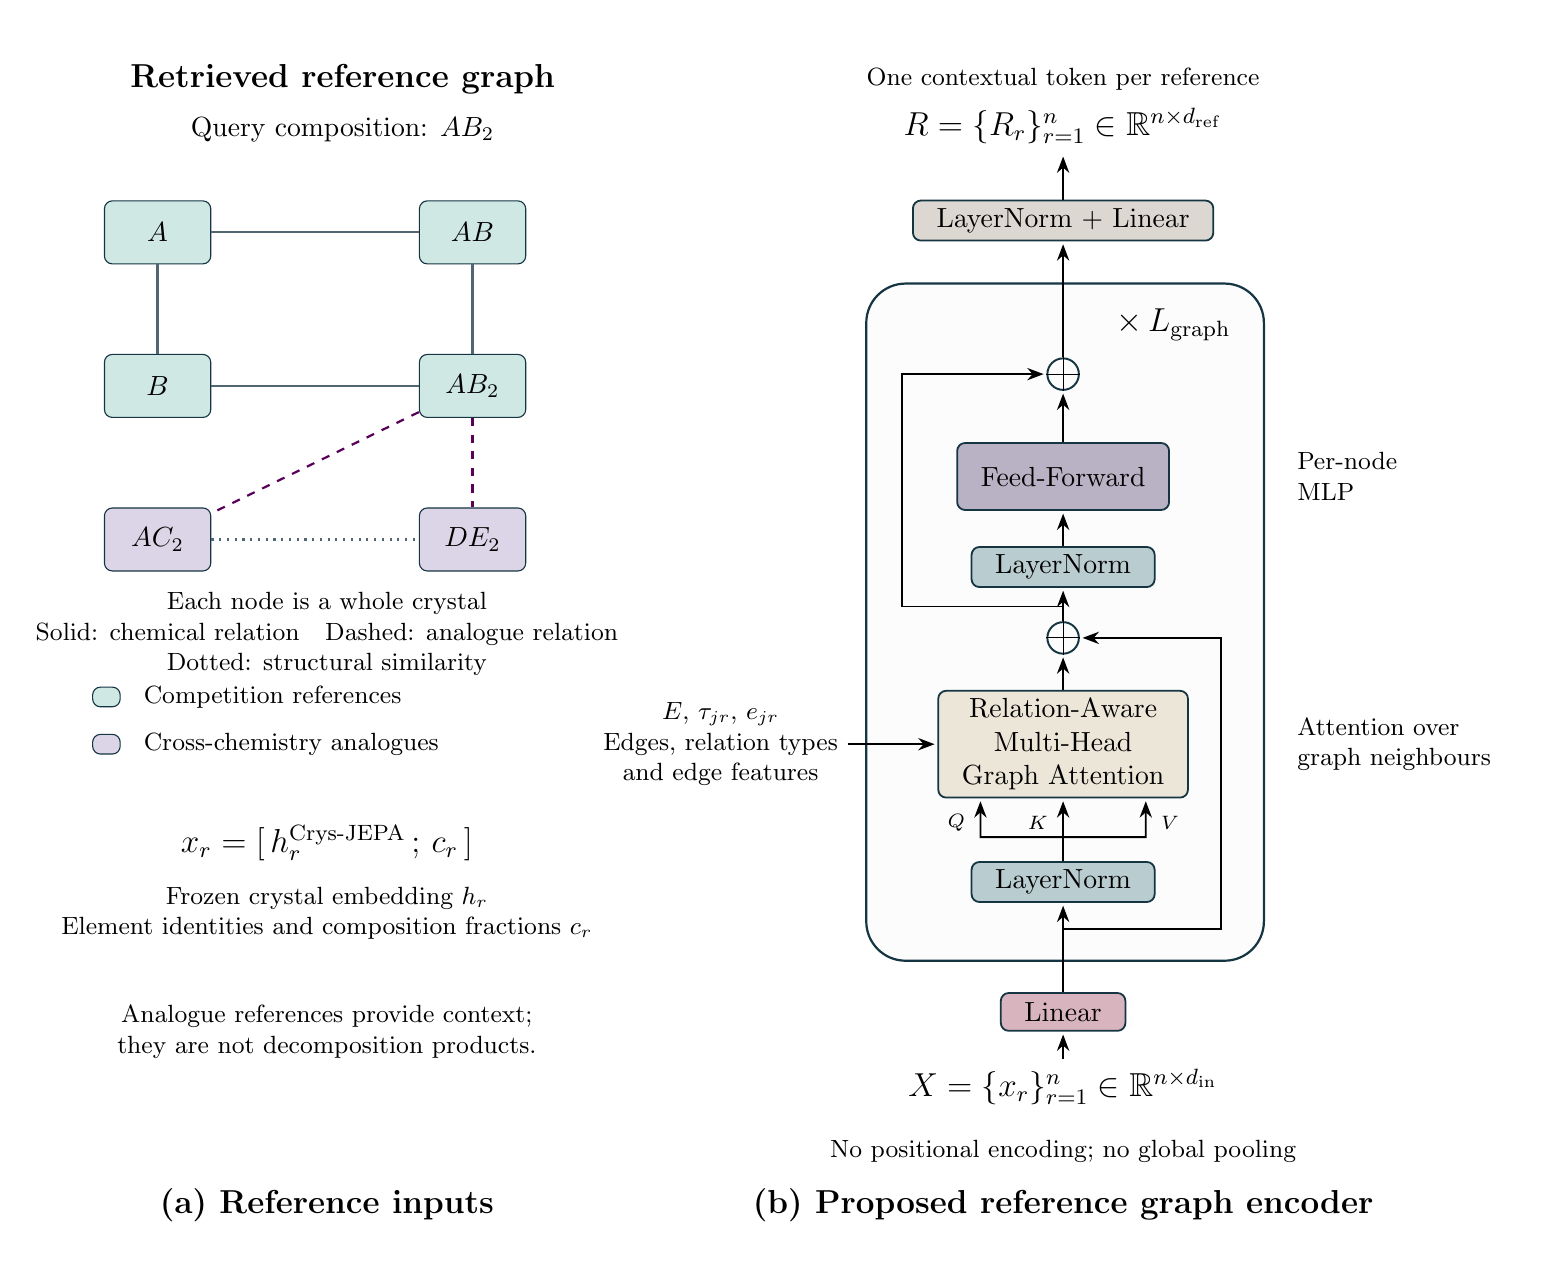
\begin{tikzpicture}[x=1cm,y=1cm,>=Stealth,
 every node/.style={font=\normalsize},
 layer/.style={draw=outline,line width=.65pt,rounded corners=1mm,align=center,minimum height=.48cm,inner xsep=3mm,inner ysep=1mm},
 arrow/.style={->,line width=.65pt,shorten >=1pt},
 add/.style={circle,draw=outline,line width=.7pt,minimum size=4mm,inner sep=0pt},
 ref/.style={draw=outline,rounded corners=1mm,minimum width=1.35cm,minimum height=.8cm,fill=comp!55},
 edge/.style={draw=outline!75,line width=.8pt},
 analogue/.style={edge,dashed,draw=violet!70!black}
]
\path[use as bounding box] (0,0) rectangle (19,15.3);

% (a) Whole-crystal graph. Lines indicate relationships, not atomic bonds.
\node[font=\large\bfseries] at (4,14.65) {Retrieved reference graph};
\node at (4,14) {Query composition: $AB_2$};
\node[ref] (a) at (1.65,12.7) {$A$};
\node[ref] (ab) at (5.65,12.7) {$AB$};
\node[ref] (b) at (1.65,10.75) {$B$};
\node[ref] (ab2) at (5.65,10.75) {$AB_2$};
\node[ref,fill=analog!65] (ac) at (1.65,8.8) {$AC_2$};
\node[ref,fill=analog!65] (de) at (5.65,8.8) {$DE_2$};
\draw[edge] (a)--(ab)--(ab2)--(b)--(a);
\draw[analogue] (ab2)--(ac);
\draw[analogue] (ab2)--(de);
\draw[edge,dotted] (ac)--(de);
\node[align=center,font=\small] at (3.8,7.6) {Each node is a whole crystal\\Solid: chemical relation\quad Dashed: analogue relation\\Dotted: structural similarity};

\node[ref,minimum width=.35cm,minimum height=.25cm,inner sep=0pt] at (1.0,6.8) {};
\node[anchor=west,font=\small] at (1.35,6.8) {Competition references};
\node[ref,fill=analog!65,minimum width=.35cm,minimum height=.25cm,inner sep=0pt] at (1,6.2) {};
\node[anchor=west,font=\small] at (1.35,6.2) {Cross-chemistry analogues};
\node[font=\large] at (3.8,4.95) {$x_r=[\,h_r^{\mathrm{Crys\text{-}JEPA}}\,;\,c_r\,]$};
\node[align=center,font=\small] at (3.8,4.05) {Frozen crystal embedding $h_r$\\Element identities and composition fractions $c_r$};
\node[align=center,font=\small] at (3.8,2.55) {Analogue references provide context;\\they are not decomposition products.};

% (b) Pre-norm graph-attention encoder, in the style of the supplied paper figure.
\node[font=\large] (input) at (13.15,1.85) {$X=\{x_r\}_{r=1}^{n}\in\mathbb R^{n\times d_{\mathrm{in}}}$};
\node[layer,fill=linear] (inproj) at (13.15,2.8) {Linear};
\draw[arrow] (input)--(inproj);

\draw[draw=outline,line width=.8pt,rounded corners=5mm,fill=black!1]
 (10.65,3.45) rectangle (15.7,12.05);
\node[anchor=north east,font=\large] at (15.4,11.85) {$\times\,L_{\mathrm{graph}}$};

\node[layer,fill=norm] (norm1) at (13.15,4.45) {LayerNorm};
\node[layer,fill=attn,minimum width=3.0cm,minimum height=1.05cm] (attention) at (13.15,6.2)
 {Relation-Aware\\Multi-Head\\Graph Attention};
\node[add] (add1) at (13.15,7.55) {};
\draw (add1.west)--(add1.east) (add1.south)--(add1.north);
\node[layer,fill=norm] (norm2) at (13.15,8.45) {LayerNorm};
\node[layer,fill=ffn,minimum width=2.6cm,minimum height=.85cm] (feed) at (13.15,9.6) {Feed-Forward};
\node[add] (add2) at (13.15,10.9) {};
\draw (add2.west)--(add2.east) (add2.south)--(add2.north);
\node[layer,fill=output] (outproj) at (13.15,12.85) {LayerNorm + Linear};
\node[font=\large] (tokens) at (13.15,14.05) {$R=\{R_r\}_{r=1}^{n}\in\mathbb R^{n\times d_{\mathrm{ref}}}$};
\node[font=\small] at (13.15,14.65) {One contextual token per reference};

\draw[arrow] (inproj)--(norm1);
% Explicit Q, K, V branches refer to normalized node states.
\draw[arrow] (norm1.north)--(attention.south);
\draw[arrow] (13.15,5.02)--(12.1,5.02)--([xshift=-10.5mm]attention.south);
\draw[arrow] (13.15,5.02)--(14.2,5.02)--([xshift=10.5mm]attention.south);
\node[font=\scriptsize,anchor=east] at (12.03,5.2) {$Q$};
\node[font=\scriptsize,anchor=east] at (13.08,5.2) {$K$};
\node[font=\scriptsize,anchor=west] at (14.27,5.2) {$V$};
\draw[arrow] (attention)--(add1);
\draw[arrow] (add1)--(norm2);
\draw[arrow] (norm2)--(feed);
\draw[arrow] (feed)--(add2);
\draw[arrow] (add2)--(outproj);
\draw[arrow] (outproj)--(tokens);
% Residual paths, routed around the layers.
\draw[arrow] (13.15,3.85)--(15.15,3.85)|-(add1.east);
\draw[arrow] (13.15,7.95)--(11.1,7.95)|-(add2.west);

% Side inputs are edge information, not an additional crystal encoder.
\node[align=center,font=\small] (edges) at (8.8,6.2) {$E,\,\tau_{jr},\,e_{jr}$\\Edges, relation types\\and edge features};
\draw[arrow] (edges.east)--(attention.west);
\node[align=left,font=\small,anchor=west] at (16.0,6.2) {Attention over\\graph neighbours};
\node[align=left,font=\small,anchor=west] at (16.0,9.6) {Per-node\\MLP};
\node[align=center,font=\small] at (13.15,1.03) {No positional encoding; no global pooling};

\node[font=\large\bfseries] at (3.8,.35) {(a) Reference inputs};
\node[font=\large\bfseries] at (13.15,.35) {(b) Proposed reference graph encoder};
\end{tikzpicture}
\end{document}
